\documentclass[a4paper,14pt]{article}


%%% Работа с русским языком
\usepackage{cmap}					% поиск в PDF
\usepackage[T2A]{fontenc}			% кодировка
\usepackage[utf8]{inputenc}		% кодировка исходного текста
\usepackage[russian]{babel}	% локализация и переносы
%\usepackage{pscyr}
%\renewcommand{\rmdefault}{ftm}
%%% Дополнительная работа с математикой
\usepackage{amsmath,amsfonts,amssymb,amsthm,mathtools} % AMS
% Please add the following required packages to your document preamble:
\usepackage{booktabs}
%% Номера формул
%\mathtoolsset{showonlyrefs=true} % Показывать номера только у тех формул, на которые есть \eqref{} в тексте.
%\usepackage{leqno} % Нумерация формул слева
%\usepackage{rumathgrk1}
%% Перенос знаков в формулах (по Львовскому)
\newcommand*{\hm}[1]{#1\nobreak\discretionary{}
	{\hbox{$\mathsurround=0pt #1$}}{}}
%\usepackage{glonti}
%%% Работа с картинками
\usepackage{graphicx}  % Для вставки рисунков
\graphicspath{{images/}{images2/}}  % папки с картинками
% \usepackage{wrapfig} % Обтекание рисунков текстом
\addto\captionsrussian{\def\refname{Список используемой литературы}}
%%% Работа с таблицами
\usepackage{array,tabularx,tabulary} % Дополнительная работа с таблицами
\usepackage{longtable}  % Длинные таблицы
\usepackage{multirow} % Слияние строк в таблице
%%% Теоремы
\theoremstyle{plain} % Это стиль по умолчанию, его можно не переопределять.
\newtheorem{theorem}{Теорема}[section]
\newtheorem{proposition}[theorem]{Утверждение}

\theoremstyle{definition} % "Определение"
\newtheorem{corollary}{Следствие}[theorem]
\newtheorem{problem}{Задача}[section]

\theoremstyle{remark} % "Примечание"
\newtheorem*{nonum}{Решение}
%\pagestyle{empty}
%%% Страница
\usepackage{extsizes} % Возможность сделать 14-й шрифт
\usepackage{geometry} % Простой способ задавать поля
\geometry{top=20mm}
%\geometry{bottom=35mm}
\geometry{left=25mm}
\geometry{right=20mm}
\setlength{\parindent}{1.1cm}

\usepackage{setspace} % Интерлиньяж
\onehalfspacing % Интерлиньяж 1.5
% \doublespacing % Интерлиньяж 2
%\singlespacing % Интерлиньяж 1

\usepackage{lastpage} % Узнать, сколько всего страниц в документе.
\usepackage[usenames]{color}
\usepackage{colortbl}
\renewcommand{\baselinestretch}{1.05}
\usepackage{hyperref}
\usepackage[usenames,dvipsnames,svgnames,table]{xcolor}
\hypersetup{				% Гиперссылки
	unicode=true,           % русские буквы в раздела PDF
	pdftitle={Заголовок},   % Заголовок
	pdfauthor={Автор},      % Автор
	pdfsubject={Тема},      % Тема
	pdfcreator={Создатель}, % Создатель
	pdfproducer={Производитель}, % Производитель
	pdfkeywords={keyword1} {key2} {key3}, % Ключевые слова
	colorlinks=true,       	% false: ссылки в рамках; true: цветные ссылки
	linkcolor=black,          % внутренние ссылки
	citecolor=blue,        % на библиографию
	filecolor=magenta,      % на файлы
	urlcolor=cyan           % на URL
}

\usepackage{bm}

\begin{document}
% НАЧАЛО ТИТУЛЬНОГО ЛИСТА
\begin{center}
    {\textsc{Федеральное государственное бюджетное образовательное
            учреждение высшего образования
        }}\\
    {\textsc{Московский государственный университет имени М.В. Ломоносова
    }} \\
    \vspace{0.2cm}
    {\textsc{Механико - математический факультет}}\\
    \vspace{0.2cm}
    {\textsc{Кафедра прикладной механики и управления}}\\
    \hfill \break
    \begin{figure}[h!]
        \centering
        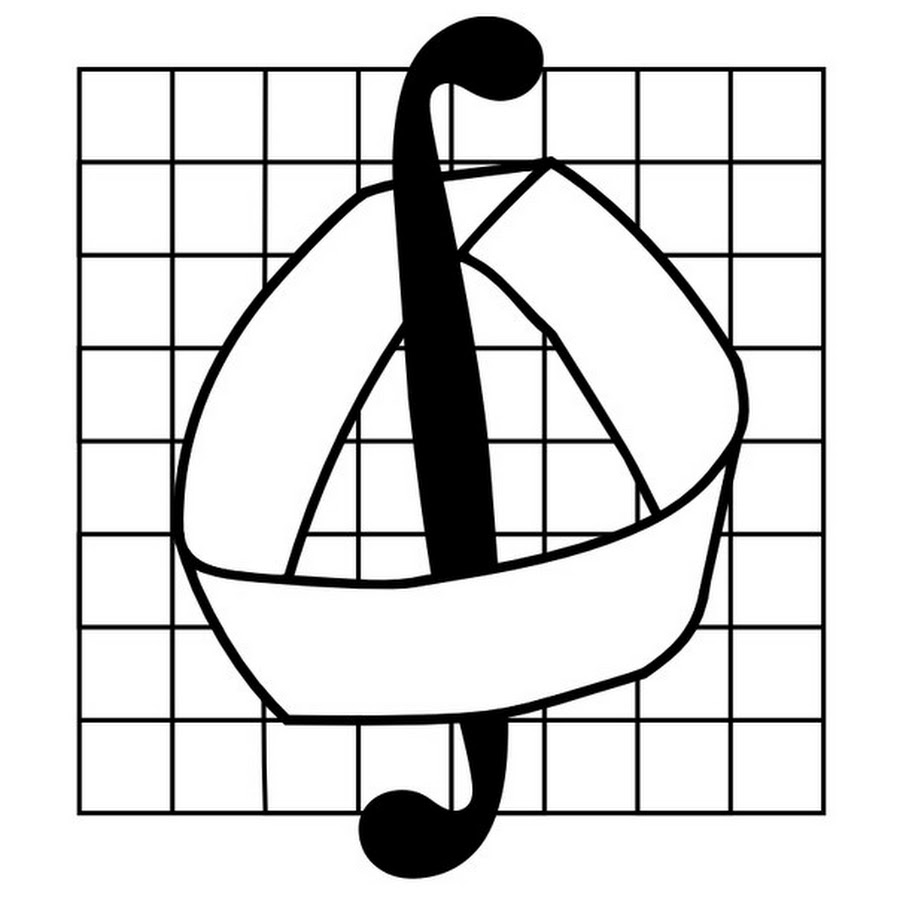
\includegraphics[width=0.30\linewidth]{emblema}
        \label{fig:emblema}
    \end{figure}
    \hfill \break
    \hfill \break
    \large{\textbf{Курсовая работа}\\
        \hfill \break Модель восстановления человеком исходной позы после толчка
    }
\end{center}

\hfill \break
\hfill \break
\begin{flushright}
    {
        Выполнил: студент группы М -- 1 \\ Романов Андрей Владимирович}
\end{flushright}

\begin{flushright}
    {
        Научный руководитель: к.ф.-м.н., \\ Кручинин Павел Анатольевич}
\end{flushright}
\hfill \break
\hfill \break
\begin{center} {Москва, 2022} \end{center}



\thispagestyle{empty} % выключаем отображение номера для этой страницы
\normalsize{
% КОНЕЦ ТИТУЛЬНОГО ЛИСТА
\newpage
\tableofcontents
\newpage

\section{Введение}
В литературе встречается решение задач оптимального быстродействия для моделей движения человека \cite{pandy,humanMovements}. Исследование таких задач может помочь объяснить некоторые особенности результатов, наблюдаемых при обследованиях.
Проба со ступенчатым воздействием является одной из стандартных проб
при стабилометрических исследованиях \cite{AdaptFizkult,stabilographTest}. При проведении этой пробы
обследуемый стоит на платформе стабилоанализатора перед экраном, на
котором изображена мишень и отображается движение центра давления
человека, после толчка в спину, определяемое по показаниям стабилоанализатора.

В ходе теста производят толкающее воздействие на человека с помощью руки или
груза, помещенного на подвижном отвесе \cite{pusher}. В результате внешнего
воздействия тело человека наклоняется вперед и при не очень сильном толчке
он не теряет равновесие и не падает, а возвращается в исходное
положение за счет изменения угла в голеностопном суставе. Изменение
остальных суставных углов может оказаться тоже не столь значительным.
Родственные задачи уже решались в работах \cite{PAKrychinin,kasatkin}.
Схематическое изображение эксперимента представлено на рисунке \ref{fig:pusher}.
\begin{figure}[h!]
    \centering
    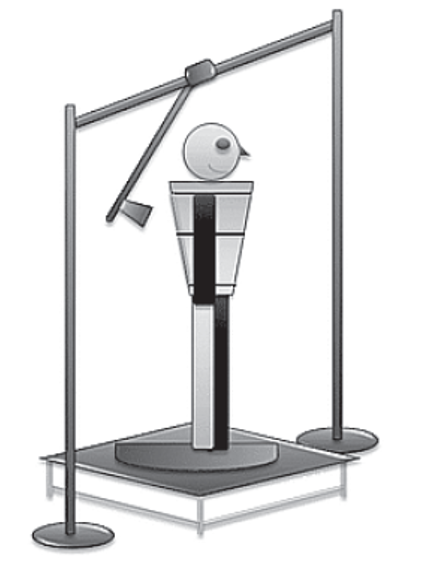
\includegraphics[]{human.png}
    \caption{Cхематическое изображение толкателя и
        положения испытуемого на стабилоплатформе}
    \label{fig:pusher}
\end{figure}

Исходные данные об отклонении сагиттальной коордианты при различных по силе толчках, предоставлены сотрудниками ИМБП РАН (см. рисунок \ref{fig:pushes})
\begin{figure}[h!]
    \centering
    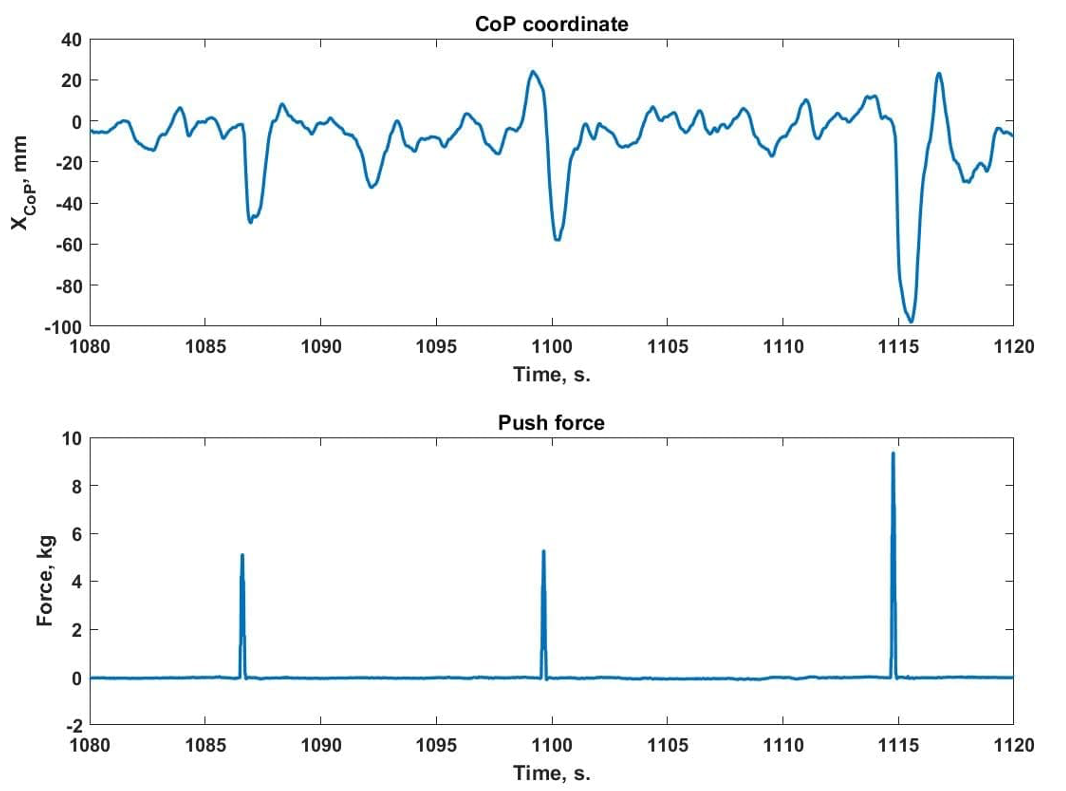
\includegraphics[width=0.9\linewidth]{Pushes.png}
    \caption{Отклонение сагиттальной координаты при различных по силе толчках}
    \label{fig:pushes}
\end{figure}

В курсовой работе предполагается рассмотреть возможные
алгоритмы управления изменением позы человека, основанные на решении задачи
оптимального быстродействия, которые можно было бы использовать для
возвращения человека в исходную вертикальную позу. В качестве математической модели
используется модель «перевернутого маятника»\cite{PAKrychinin,kasatkin,gurfincel}. В дальнейшем
такое решение предполагается использовать для оценки эффективности управления человеком
при возвращении в вертикальную позу, путем сравнения
времени реального процесса с полученным эталонным решением оптимальной задачи.

\newpage
\section{Математическая модель и постановка задачи управления}
Для описания движения тела человека в сагиттальной плоскости используем традиционную модель перевернутого маятника (см. рисунок \ref{fig:pendulum}).

\begin{figure}[h!]
    \centering
    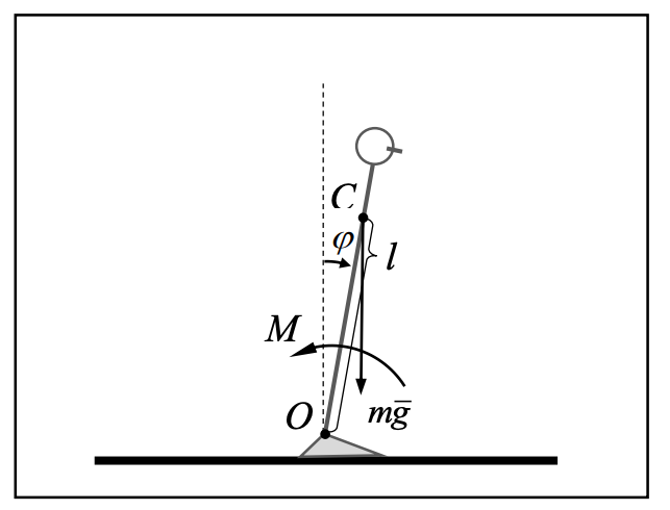
\includegraphics[width=0.9\linewidth]{pendulum.png}
    \caption{Модель перевернутого маятника}
    \label{fig:pendulum}
\end{figure}

Традиционно предполагаем, что тело человека в ходе теста допустимо
моделировать недеформируемым однородным стержнем массы $m$,
закрепленным шарнирно в точке $O$, которая соответствует
голеностопному суставу.

Центр масс стержня расположен в точке $C$, удаленной от точки $O$
на расстояние $l$. Момент инерции стержня относительно фронтальной
оси, проходящей через точку $O$, равен $J$. Отклонение стержня от
вертикали описывается углом $\varphi$. Будем считать, что обследуемый
ориентирован так, что его сагиттальная плоскость параллельна оси
чувствительности платформы, а его стопа неподвижна относительно
платформы. Скорость изменения момента $M$, который приложен в точке $O$ к стержню,
будем считать управлением.

Уравнение моментов для малых значений угла $\varphi$ и
скорости его изменения запишем, как традиционно принято для этой задачи.
\[
    J\ddot{\varphi}= m_Tgl\varphi+M
\]

Необходимо перевести решение уравнения из начального состояния
\[
    \varphi(0)=\varphi_0, \,\dot{\varphi}(0)=\omega_0
\]

в конечное состояние
\[
    \varphi(t_k)=\varphi_k,\, \dot{\varphi}(t_k)=0.
\]

Перевод состояния тела должен происходить за минимальное
время $t_k$, с помощью изменений значения $\dot{M}$ в
голеностопном суставе.

Будем принимать во внимание условия ограниченности скорости изменения
момента в голеностопном суставе
\[
    U^-\leqslant\dot{M}\leqslant\ U^+.
\]

Будем считать, что за время толчка нервная система человека
не успела среагировать и момент в голеностопном суставе остался
неизменным и соответствует значению, обеспечивающему положение
равновесия человека до начала движения и после его завершения
\[
    M(0)=M\left(t_k\right)=-m_Tgl\varphi_k;
\]

Для дальнейшего анализа задачи представим приведенные
соотношения в безразмерном виде. Для этого перейдем
к новым переменным
\[
    \theta=\frac{\varphi-\varphi_k}{\varphi_\ast},\ \ m=\frac{M-M_f}{m_Tgl\varphi_\ast}.
\]

В качестве характерного значения угла выберем разность
начального и конечного значений угла в голеностопном
суставе при выполнении пробы $\varphi_\ast=\varphi_0-\varphi_k$

Введем безразмерное время
\[
    \tau=\frac{t}{t_\ast},\ t_\ast=\sqrt{\frac{J}{m_Tgl}}.
\]

Управлением $u$ будем считать скорость изменения безразмерного
момента. Для этих переменных обезразмеренные уравнения движения
примут следующий вид
\begin{equation}\label{system}
    \theta^{''}=\theta+m;\ m^{'}=u
\end{equation}

Здесь через $m^{'}$ обозначено дифференцирование по
безразмерному времени $\tau$. Необходимо решение системы \eqref{system}
перевести из начального положения
\[
    \theta(0)=1;\ \theta^{'}(0)=\frac{t_\ast}{\varphi_\ast}\omega_0=\Omega_0;\ m(0)=0
\]
в положение
\[
    \theta(\tau_f)=0;\ \theta^{'}(\tau_f)=0;\ m(\tau_f)=0
\]
с помощью ограниченного управления
\[
    u^-\leqslant\ u\leqslant\ u^+,\ \text{где}
\]
\[
    u^-=\frac{U^-}{mgl\varphi_\ast t_\ast},\ \ u^+=\frac{U^+}{mgl\varphi_\ast t_\ast}.
\]
Далее будем считать, что $u^-=-u^+$
\newpage
\section{Задача оптимального быстродействия при ограничении на величину скорости изменения момента}
Выпишем систему в форме Коши
\begin{equation}\label{koshisystem}
    \left\{ {\begin{aligned}
                 & \theta^{'} = \omega , \hfill   \\
                 & \omega^{'} = \theta+m , \hfill \\
                 & m^{'} = u . \hfill             \\
            \end{aligned}} \right.
\end{equation}

$|u|\leqslant u_{max}$
\[
    \theta(0)=1;\ \omega(0)=\frac{t_\ast}{\varphi_\ast}\omega_0=\Omega_0;\ m(0)=0
\]
\[
    \theta(\tau_f)=0;\ \theta^{'}(\tau_f)=0;\ m(\tau_f)=0
\]
$J=\tau_f\to \min$

Для решения задачи оптимального быстродействия будем использовать принцип максимума Понтрягина \cite{Optimal}:

Если $\{y^0(\cdot),u^0(\cdot),[t_0,t_k^0]\} - $ оптимальный процесс, то существует нетривиальная пара $\{\lambda_0\geq0,\psi(\cdot)\}$
такая, что
\begin{itemize}
    \item $ \mathop {\max }\limits_{u(t) \in \Omega}  H(\psi(t),y^0(t),u(t))=H(\psi(t),y^0(t),u^0(t))$
          $\forall t \in T \subseteq [t_0,t_k^0];$
    \item $\psi(t_k^0)+\lambda_0(\frac{\partial \varphi_0(y^0(t_k^0))}{\partial y})^T \perp M \text{ в точке } y^0(t_k^0);$
    \item $\mathcal{H}=H(\psi(t),y^0(t),u^0(t))\equiv0 \text{ при } t \in [t_0,t_k^0].$
\end{itemize}
Запишем функцию Понтрягина
\[
    H(\psi(t),y(t),u(t))=\psi_1\cdot\omega+\psi_2\cdot(\theta+m)+\psi_3\cdot u
\]
Сопряженная система уравнений:
\[
    \psi^{'}_i  =  - \frac{{\partial H}}{{\partial y_i }},\,\,i = 1, \ldots ,n
\]
В данной задаче $y_1 = \theta, y_2 = \omega, y_3=m$, тогда сопряженная система примет вид
\begin{equation} \label{7}
    \left\{ {\begin{aligned}
                 & \psi^{'}_1=  - \frac{{\partial H}}{{\partial \theta}} = - \psi_2\hfill  \\
                 & \psi^{'}_2=  - \frac{{\partial H}}{{\partial \omega }} = - \psi_1\hfill \\
                 & \psi^{'}_3=  - \frac{{\partial H}}{{\partial m }} = - \psi_2 \hfill     \\
            \end{aligned}} \right.
\end{equation}
При $\psi_3\equiv0$ следует, что $\psi_2\equiv0$ и $\psi_1\equiv0$ следовательно особого управления нет.

Тогда для условия максимизации функции Понтрягина
\[
    u=
    \begin{cases}
        -u_{max}, & \text{при $\psi_3<0$}          \\
        +u_{max}, & \text{при $\psi_3\geqslant 0$}
    \end{cases}
\]\\*
Продифференцируем по безразмерному времени второе уравнение из \eqref{7} и подставим в него первое, получим
\[
    \psi_2 ''=\psi_2
\]
Решая систему \eqref{7}, получим
\[
    \left\{ {\begin{aligned}
                 & \psi_1 = -C_1e^\tau+C_2e^{-\tau}+C_3, \hfill  \\
                 & \psi_2 = C_1e^\tau+C_2e^{-\tau} , \hfill      \\
                 & \psi_3 = -C_1e^\tau+C_2e^{-\tau}+C_3 . \hfill \\
            \end{aligned}} \right.
\]

Анализируя корни уравнения $\psi_3(\tau)=0$, для различной комбинации
коэффициентов $C_1,C_2,C_3$, получим, что число корней не может быть больше двух. В системе может быть не более двух переключений $u$.

Пусть $u^*=\mathrm{const}$ управление на первом участке траектории до первого переключения $u^*=-u_{max}$.

Решая систему \eqref{koshisystem}, получим
\begin{equation}\label{solvekoshi}
    \left\{ {\begin{aligned}
                 & m(\tau) = \tau u+C_1, \hfill                                                            \\
                 & \theta(\tau) = \frac{1}{2} e^{-\tau } \left((C_1+C_2+C_3) e^{2 \tau }-2 e^{\tau } (\tau
                u+C_1)+C_1+C_2-C_3\right), \hfill                                                          \\
                 & \omega(\tau) = \frac{1}{2} e^{-\tau } \left((C_1+C_2+C_3) e^{2 \tau }-2 e^{\tau }
                u-C_1-C_2+C_3\right). \hfill                                                               \\
            \end{aligned}} \right.
\end{equation}
\newpage
Пусть первое переключение управления происходит в момент времени
$\tau=\tau_1$, а второе в момент времени
$\tau=\tau_2$. Рассмотрим систему \eqref{koshisystem} на трех этапах,
при переходе между которыми меняется управление.

Этап 1. $u=-u_*$ начальные условия
\[
    m(0)=0;\ \theta(0)=1;\ \omega(0)=\Omega_0;
\]

Из \eqref{solvekoshi} получим
\[
    \left\{ {\begin{aligned}
                 & 0 = -\tau  u_*+c_1, \hfill                                                            \\
                 & 1 = \frac{1}{2} e^{-\tau } \left(C_1 \left(e^{\tau }-1\right)^2+C_2 \left(e^{2
                \tau }+1\right)+C_3 e^{2 \tau }-C_3+2 e^{\tau } \tau  u_*\right) , \hfill                \\
                 & \Omega_0 = \frac{1}{2} e^{-\tau } \left(C_1 \left(e^{2 \tau }-1\right)+C_2 \left(e^{2
                \tau }-1\right)+C_3 e^{2 \tau }+C_3+2 e^{\tau } u_*\right)  . \hfill                     \\
            \end{aligned}} \right.
\]
Тогда
\[
    \left\{ {\begin{aligned}
                 & C_1 = 0, \hfill             \\
                 & C_2 = 1, \hfill             \\
                 & C_3 = -u_*+\Omega_0. \hfill \\
            \end{aligned}} \right.
\]
Подставим полученные константы в \eqref{solvekoshi}
\[
    \left\{ {\begin{aligned}
                 & m_1(\tau) = -\tau  u_*, \hfill                                                                         \\
                 & \theta_1(\tau) = \frac{e^\tau+e^{-\tau}}{2}+\frac{\Omega_0-u_*}{2}(e^\tau-e^{-\tau})+\tau u_* , \hfill \\
                 & \omega_1(\tau) =\frac{e^\tau-e^{-\tau}}{2}+\frac{\Omega_0-u_*}{2}(e^\tau+e^{-\tau})+u_*   . \hfill     \\
            \end{aligned}} \right.
\]
Этап 2. $u=u_*$ начальные условия
\[
    m(\tau_1)=m_1(\tau_1); \ \theta(\tau_1)=\theta_1(\tau_1);\ \omega(\tau_1)=\omega_1(\tau_1);
\]
\[
    \left\{ {\begin{aligned}
                 & m(\tau_1) = -\tau _1 u_*, \hfill                                                            \\
                 & \theta(\tau_1) = \frac{1}{2} e^{-\tau _1} \left(\left(e^{2 \tau _1}-1\right) \Omega _0+e^{2
                \tau _1}+\left(2 e^{\tau _1} \tau _1-e^{2 \tau _1}+1\right) u_*+1\right) , \hfill              \\
                 & \omega(\tau_1) = \frac{1}{2} e^{-\tau _1} \left(\left(e^{2 \tau _1}+1\right) \Omega
                _0-\left(e^{\tau _1}-1\right) \left(-e^{\tau _1}+\left(e^{\tau
                _1}-1\right) u_*-1\right)\right) . \hfill                                                      \\
            \end{aligned}} \right.
\]
Находим константы интегрирования
\[
    \left\{ {\begin{aligned}
                 & -\tau _1 u_* = \tau _1 u_*+C_1, \hfill                                         \\
                 & \frac{1}{2} e^{-\tau _1} \left(\left(e^{2 \tau _1}-1\right) \Omega _0+e^{2
                \tau _1}+\left(2 e^{\tau _1} \tau _1-e^{2 \tau _1}+1\right) u_*+1\right) =        \\
                 & = \frac{1}{2} e^{-\tau _1} \left(C_1 \left(e^{\tau _1}-1\right){}^2+C_2 e^{2
                \tau _1}+C_3 e^{2 \tau _1}-2 e^{\tau _1} \tau _1 u_*+C_2-C_3\right) , \hfill      \\
                 & \frac{1}{2} e^{-\tau _1} \left(\left(e^{2 \tau _1}+1\right) \Omega
                _0-\left(e^{\tau _1}-1\right) \left(-e^{\tau _1}+\left(e^{\tau
                _1}-1\right) u_*-1\right)\right)=                                                 \\
                 & =\frac{1}{2} e^{-\tau _1} \left(C_1 \left(e^{2 \tau _1}-1\right)+C_2 e^{2 \tau
                _1}+C_3 e^{2 \tau _1}-2 e^{\tau _1} u_*-C_2+C_3\right)  . \hfill                  \\
            \end{aligned}} \right.
\]
\[
    \left\{ {\begin{aligned}
                 & C_1 =-2 \tau _1 u_*, \hfill                                                    \\
                 & C_2 = -e^{-\tau _1} \left(-e^{\tau _1}+e^{2 \tau _1} u_*-2 e^{\tau _1} \tau _1
                u_*-u_*\right), \hfill                                                            \\
                 & C_3 = e^{-\tau _1} \left(e^{\tau _1} \Omega _0-e^{\tau _1} u_*+e^{2 \tau _1}
                u_*+u_*\right). \hfill                                                            \\
            \end{aligned}} \right.
\]

Подставим начальные условия для второго этапа в \eqref{solvekoshi}, получим

\[
    \left\{ {\begin{aligned}
                 & m_2(\tau) = \left(\tau -2 \tau _1\right) u_*, \hfill                                                                                                \\
                 & \theta_2(\tau) = \frac{e^\tau+e^{-\tau}}{2}+\frac{\Omega_0-u_\ast}{2}(e^\tau-e^{-\tau})+u_*(e^{\tau-\tau_1}-e^{-\tau+\tau_1}+2\tau_1-\tau) , \hfill \\
                 & \omega_2(\tau) = \frac{e^\tau-e^{-\tau}}{2}+\frac{\Omega_0-u_\ast}{2}(e^\tau+e^{-\tau})+u_*(e^{\tau-\tau_1}+e^{-\tau+\tau_1}-1) . \hfill            \\
            \end{aligned}} \right.
\]
Этап 3. $u=-u_*$ конечные условия
\[
    m(\tau_f)=0; \ \theta(\tau_f)=0;\ \omega(\tau_f)=0;
\]
Подставим начальные условия в \eqref{solvekoshi}, получим
\[
    \left\{ {\begin{aligned}
                 & 0 = C_1-\tau_f  u_*, \hfill                                               \\
                 & 0 = \frac{1}{2} e^{-\tau _f} \left(C_1 \left(e^{\tau _f}-1\right){}^2+C_2
                \left(e^{2 \tau _f}+1\right)+C_3 e^{2 \tau _f}-C_3+2 u_* e^{\tau _f} \tau
                _f\right), \hfill                                                            \\
                 & 0 = \frac{1}{2} e^{-\tau _f} \left(C_1 \left(e^{2 \tau _f}-1\right)+C_2
                \left(e^{2 \tau _f}-1\right)+C_3 e^{2 \tau _f}+C_3+2 u_* e^{\tau
                _f}\right)  . \hfill                                                         \\
            \end{aligned}} \right.
\]
\[
    \left\{ {\begin{aligned}
                 & C_1 = u_* \tau _f, \hfill                                                  \\
                 & C_1 = \frac{1}{2} u_* e^{-\tau _f} \left(-2 e^{\tau _f} \tau _f+e^{2 \tau
                _f}-1\right), \hfill                                                          \\
                 & C_2 = -\frac{1}{2} u_* e^{-\tau _f} \left(e^{2 \tau _f}+1\right)  . \hfill \\
            \end{aligned}} \right.
\]
Тогда решение на этом этапе имеет вид
\[
    \left\{ {\begin{aligned}
                 & m_3(\tau) = u_* \left(\tau _f-\tau \right), \hfill                                           \\
                 & \theta_3(\tau) = \frac{1}{2} u_* \left(-e^{\tau -\tau _f}+e^{\tau _f-\tau }-2 \tau _f+2 \tau
                \right), \hfill                                                                                 \\
                 & \omega_3(\tau) =u_*-\frac{u_*}{2}(e^{\tau-\tau_f}+e^{-\tau+\tau_f}) . \hfill                 \\
            \end{aligned}} \right.
\]
Теперь найдем решения, учитывая что
\[
    \left\{ {\begin{aligned}
                 & m_2(\tau_2) = m_3(\tau_2), \hfill            \\
                 & \theta_2(\tau_2) =  \theta_3(\tau_2), \hfill \\
                 & \omega_2(\tau_2) = \omega_3(\tau_2) . \hfill \\
            \end{aligned}} \right.
\]
Получим
\[
    \left\{
    \begin{multlined}
        \left(\tau _2-2 \tau _1\right) u_*=u_* \left(\tau _f-\tau _2\right), \\
        % 2-nd equation
        \shoveleft{\frac{e^{\tau_2}+e^{-\tau_2}}{2}+\frac{\Omega_0-u_\ast}{2}(e^{\tau_2}-e^{-\tau_2})+u_*(e^{\tau_2-\tau_1}-e^{-\tau_2+\tau_1}+2\tau_1-\tau_2)=} \\
        \shoveleft{=\frac{1}{2} u_* \left(-e^{\tau _2-\tau _f}+e^{\tau _f-\tau _2}-2 \tau _f+2
            \tau _2\right),} \\
        % 4-th equation
        \shoveleft{\frac{e^{\tau_2}-e^{-\tau_2}}{2}+\frac{\Omega_0-u_\ast}{2}(e^{\tau_2}+e^{-\tau_2})+u_*(e^{\tau_2-\tau_1}+e^{-\tau_2+\tau_1}-1)=} \\
        \shoveleft{=u_*-\frac{u_*}{2}(e^{\tau_2-\tau_f}+e^{-\tau_2+\tau_f}).} \\
    \end{multlined}
    \right.
\]

Сократим первое уравнение на $u_*$, выражение для $\tau_f$ из первого уравнения подставим во второе и третье
\begin{equation}\label{fullconnected}
    \left\{ {\begin{aligned}
                 & \tau_f=2(\tau_2-\tau_1),                                                                                                                                                                 \\
                 & \frac{e^{\tau_2}+e^{-\tau_2}}{2}+\frac{\Omega_0-u_*}{2}(e^{\tau_2}-e^{-\tau_2})+u_*\left(e^{-\tau_1+\tau_2}-e^{\tau_1-\tau_2}+\frac{e^{\tau_2-\tau_f}-e^{-\tau_2+\tau_f}}{2}\right)=0,   \\
                 & \frac{e^{\tau_2}-e^{-\tau_2}}{2}+\frac{\Omega_0-u_*}{2}(e^{\tau_2}+e^{-\tau_2})+u_*\left(e^{\tau_1-\tau_2}+e^{-\tau_1+\tau_2}+\frac{e^{\tau_2-\tau_f}+e^{-\tau_2+\tau_f}}{2}-2\right)=0. \\
            \end{aligned}} \right.
\end{equation}

Введем замену переменных
\[
    x=e^{\tau_1} ,\,\,y=e^{\tau_2} ,\,\,z=e^{\frac{\tau_f}{2}}
\]
\[
    \left\{ {\begin{aligned}
                 & z=\frac{y}{x}, \hfill                                                         \\
                 & \frac{1}{2} \left(u_* \left(\frac{x^2}{y}-\frac{y}{x^2}-\frac{2 x}{y}+\frac{2
                        y}{x}-y+\frac{1}{y}\right)+\left(y-\frac{1}{y}\right) \Omega
                _0+y+\frac{1}{y}\right)=0, \hfill                                                \\
                 & \frac{u_* \left(\frac{y^2}{x^2}+x^2+\frac{2 y^2}{x}+2 x-y^2-4
                y-1\right)+\left(y^2+1\right) \Omega _0+y^2-1}{2 y}=0. \hfill                    \\
            \end{aligned}} \right.
\]
\begin{equation}\label{fullchanged}
    \left\{ {\begin{aligned}
                 & z=\frac{y}{x}, \hfill                                                                                                              \\
                 & (\Omega_0-u_*)\left( xy-\frac{x}{y}\right)+u_*\left(\frac{x^3}{y}-\frac{y}{x}-\frac{2x^2}{y}+2y\right)+\frac{x}{y}+xy=0, \hfill    \\
                 & (\Omega_0-u_*)\left( xy+\frac{x}{y}\right)+u_*\left(\frac{x^3}{y}+\frac{y}{x}+\frac{2x^2}{y}+2y-4x\right)-\frac{x}{y}+xy=0. \hfill \\
            \end{aligned}} \right.
\end{equation}
\begin{equation}\label{fullchanged1}
    \left\{ {\begin{aligned}
                 & y=zx, \hfill                                                                                                              \\
                 & (\Omega_0-u_*)\left( x^2z-\frac{x}{zx}\right)+u_*\left(\frac{x^3}{zx}-\frac{zx}{x}-\frac{2x^2}{zx}+2zx\right)+\frac{x}{zx}+x^2z=0, \hfill    \\
                 & (\Omega_0-u_*)\left( x^2z+\frac{x}{zx}\right)+u_*\left(\frac{x^3}{zx}+\frac{zx}{x}+\frac{2x^2}{zx}+2zx-4x\right)-\frac{x}{zx}+x^2z=0. \hfill \\
            \end{aligned}} \right.
\end{equation}
\begin{equation}\label{fullchanged1}
    \left\{ {\begin{aligned}
                 & (\Omega_0-u_*)\left( x^2z-\frac{1}{z}\right)+u_*\left(\frac{x^2}{z}-z-\frac{2x}{z}+2zx\right)+\frac{1}{z}+x^2z=0, \hfill    \\
                 & (\Omega_0-u_*)\left( x^2z+\frac{1}{z}\right)+u_*\left(\frac{x^2}{z}+z+\frac{2x}{z}+2zx-4x\right)-\frac{1}{z}+x^2z=0. \hfill \\
            \end{aligned}} \right.
\end{equation}
Сложим и вычтем уравнения системы
\begin{equation}\label{fullchanged2}
    \left\{ {\begin{aligned}
                 & 2(\Omega_0-u_*)x^2z+u_*\left(2\frac{x^2}{z}+4zx-4x\right)+2x^2z=0, \hfill    \\
                 & 2(\Omega_0-u_*)\frac{1}{z}+u_*\left(2z+\frac{4x}{z}-4x\right)-\frac{2}{z}=0. \hfill    \\
            \end{aligned}} \right.
\end{equation}
\begin{equation}\label{fullchanged2}
    \left\{ {\begin{aligned}
                 & 2(\Omega_0-u_*)x^2z+u_*\left(2\frac{x^2}{z}+4zx-4x\right)+2x^2z=0, \hfill    \\
                 & 2(\Omega_0-u_*)\frac{1}{z}+2u_*z+4x\left(\frac{u_*}{z}-u_*\right)-\frac{2}{z}=0. \hfill    \\
            \end{aligned}} \right.
\end{equation}
\begin{equation}\label{fullchanged2}
    \left\{ {\begin{aligned}
                 & 2(\Omega_0-u_*)x^2z+u_*\left(2\frac{x^2}{z}+4zx-4x\right)+2x^2z=0, \hfill    \\
                 & x=\left( \frac{1}{2z}-\frac{u_*z}{2}-(\Omega_0-u_*)\frac{1}{2z}\right)\frac{z}{u_*(1-z)} \hfill    \\
            \end{aligned}} \right.
\end{equation}
\[
    \frac{\left(u_* \left(z^2-1\right)+\Omega _0-1\right) \left(-u_* \left(z^4+\Omega _0 \left(z^2-1\right)^2\right)+u_*^2 (z-1)^4+u_*-\Omega _0^2 z^2+z^2\right)}{2 u_*^2 (z-1)^2}=0
\]
\begin{equation}\label{fullchanged2}
    \left[ {\begin{aligned}
                 & \left(u_* \left(z^2-1\right)+\Omega _0-1\right)=0, \hfill    \\
                 & -u_* \left(z^4+\Omega _0 \left(z^2-1\right)^2\right)+u_*^2 (z-1)^4+u_*-\Omega _0^2 z^2+z^2=0 \hfill    \\
            \end{aligned}} \right.
\end{equation}
\begin{equation}\label{fullchanged2}
    \left[ {\begin{aligned}
                 & u_*z^2+\Omega _0-1-u_*=0, \hfill    \\
                 & (-u_* \Omega _0+u_*^2-u_*)z^4-4 u_*^2z^3+(2 u_* \Omega _0+6 u_*^2-\Omega _0^2+1)z^2-4 u_*^2z+-u_* \Omega _0+u_*^2+u_*=0 \hfill    \\
            \end{aligned}} \right.
\end{equation}
% \begin{equation}\label{fullchanged3}
%     \left\{ {\begin{aligned}
%                  & 2(\Omega_0-u_*)x^2z^2+u_*\left(2x^2+4z^2x-4xz\right)+2x^2z^2=0, \hfill    \\
%                  & 2(\Omega_0-u_*)+u_*\left(2z^2+4x-4xz\right)-2=0. \hfill    \\
%             \end{aligned}} \right.
% \end{equation}
% \begin{equation}\label{fullchanged3}
%     \left\{ {\begin{aligned}
%                  & 2(\Omega_0-u_*)x^2z^2+u_*\left(2x^2+4z^2x-4xz\right)+2x^2z^2=0, \hfill    \\
%                  & 2(\Omega_0-u_*)=2-u_*\left(2z^2+4x-4xz\right). \hfill    \\
%             \end{aligned}} \right.
% \end{equation}
% \begin{equation}\label{fullchanged3}
%     \left\{ {\begin{aligned}
%                  & (2-u_*\left(2z^2+4x-4xz\right))x^2z^2+u_*\left(2x^2+4z^2x-4xz\right)+2x^2z^2=0, \hfill    \\
%                  & 2(\Omega_0-u_*)=2-u_*\left(2z^2+4x-4xz\right). \hfill    \\
%             \end{aligned}} \right.
% \end{equation}
Привести систему \eqref{fullchanged} к полиномиальному виду, как это сделано в работах \cite{PAKrychinin,kurscah}, не удалось, поэтому
дальнейший анализ задачи проведем с использованием численных методов решения систем уравнений.

\newpage
\section{Численные примеры реализации оптимального управления}
Построим оптимальную траекторию, учитывая полученные соотношения для управления.

$m_T=74$кг; $l=0.88$м; $J=\frac{4ml^2}{3}$кг$\cdot$м$^2$
\[
    t_\ast=\sqrt{\frac{J}{m_Tgl}}=\sqrt{\frac{4l}{3g}}=0.346c
\]

Значение $u^*_{max}=1.65$ уже было подсчитано в работе \cite{kurscah}.
Характерное значение для $\varphi_\ast=0.087 \text{ рад}$, для $\omega_0=0.069 \text{ рад/с}$.

$\Omega_0=\frac{t_\ast}{\varphi_\ast}\omega_0=0.274$

Численно решим систему \eqref{fullchanged} используя пакет Wolfram Mathematica и
функцию NSolve, которая ищет все корни системы полиномиальных уравенений. Также сделаем отбор корней из условия, что $x>1,y>1,z>1$. Получим $\tau_1=2.12;\tau_2=4.88;\tau_f=5.51.$
Также найдем корни системы \eqref{fullchanged} при $\theta^{'}(0)=1.3\Omega_0$ и при $\theta^{'}(0)=0.7\Omega_0$.

При $\theta^{'}(0)=\Omega_0$: $\tau_1=2.12;\tau_2=4.88;\tau_f=5.51;$

При $\theta^{'}(0)=1.3\Omega_0$: $\tau_1=2.38,\tau_2=5.41,\tau_f=6.06;$

При $\theta^{'}(0)=0.7\Omega_0$: $\tau_1=2.06,\tau_2=4.74,\tau_f=5.37.$

Для полученных значений $\tau_1,\tau_2,\tau_f$ построим графики решений системы \eqref{koshisystem}.
\begin{figure}[h!]
    \centering
    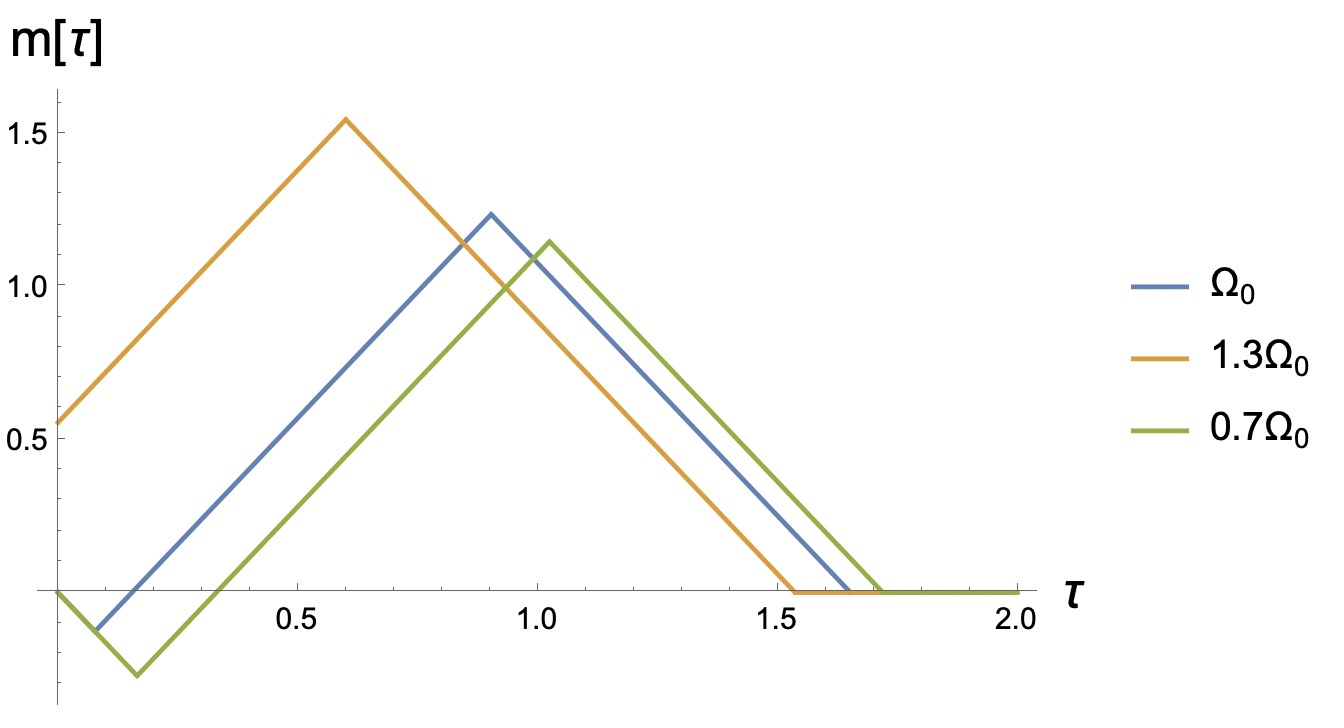
\includegraphics[width=0.69\linewidth]{m.jpeg}
    \caption{Зависимость $m(\tau)$}
    \label{fig:m}
\end{figure}
\begin{figure}[h!]
    \centering
    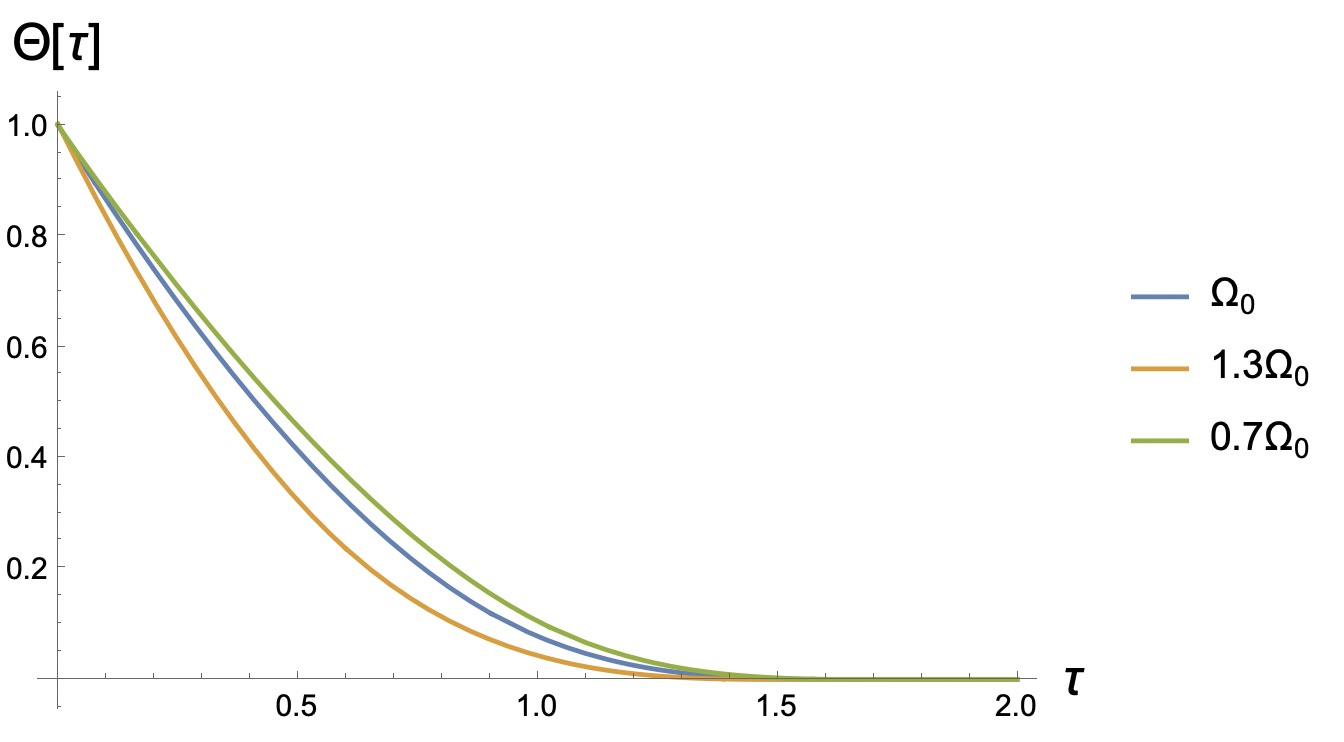
\includegraphics[width=0.69\linewidth]{theta.jpeg}
    \caption{Зависимость $\Theta(\tau)$}
    \label{fig:theta}
\end{figure}
\begin{figure}[h!]
    \centering
    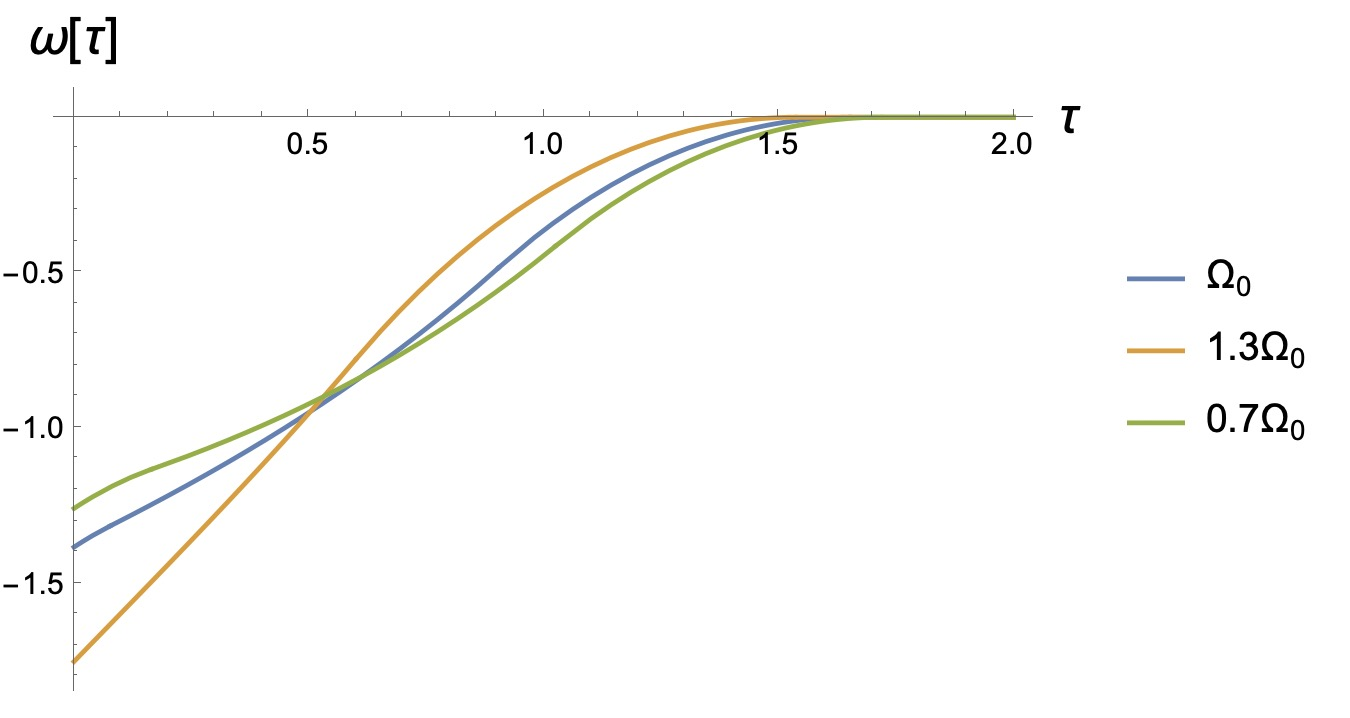
\includegraphics[width=0.69\linewidth]{omega.jpeg}
    \caption{Зависимость $\omega(\tau)$}
    \label{fig:omega}
\end{figure}


\newpage
\section{Заключение}
В курсовой работе были представлены оптимальные алгоритмы управления
движением позой при ступенчатом воздействии, основанные на модели
«перевернутого маятника» удовлетворяющие принципу максимума Понтрягина.
В задаче ставилось ограничение на скорость изменения момента в голеностопном суставе.
\begin{itemize}
    \item Показано, что решение оптимальной задачи быстродействия при ограниченной скорости изменения момента в голеностопном суставе может иметь решение, которое хорошо качественно совпадает с картиной, наблюдаемой в стабилометрических исследованиях.
    \item Время необходимое для восстановления исходной позы получилось соизмеримым с реальным времени возвращения после толчка.
\end{itemize}
\newpage
\section{Экспериментальные данные }
Экспериментальные данные  

beginPush=1130


realT=1.5;

Fmax=6.87;

Ftime=(168-155)/50;

Mom=(9.69+19.2)*m*g/1000=19.21;

theta0=0.028;

omega0=0.1767;

tast=0.1729;

///////

beginPush=1116


realT=2.0

Fmax=6.01

Ftime=(244-231)/50

Mom=(6.42+15.96)*m*g/1000=14.88

theta0=0.0292

omega0=0.149

tast=0.1729

////////

beginPush=1182


realT=1.97

Fmax=8.21

Ftime=(202-189)/50

Mom=(29-2)*m*g/1000

theta0=0.0337

omega0=0.1689

//////

beginPush=1207
realT=1.97

Fmax=8.56

Ftime=(200-187)/50

Mom=(29-0)*m*g/1000

theta0=0.0335

omega0=0.1955

///////

beginPush=1225

realT=2.5

Fmax=9.73

Ftime=(110-97)/50

Mom=(35-5)*m*g/1000

theta0=0.0359

omega0=0.2139

\begin{table}[h]
    \caption{Таблица толчков} 
    \label{tab:example}
    \small
    \centering
    \begin{tabular}{|l|c|c|c|c|c}
    \midrule
    \textbf{} & \textbf{Fmax(Н)} & \textbf{Время толчка(сек)} & \textbf{ $\phi_0$} \textbf{$\omega_0$} & \textbf{Момент после толчка(кг*м)} & \\ 
    \midrule
    Item 1 & Item 2 & Item 3 & Item 4 \\
    \midrule
    Item 1 & Item 2 & Item 3 & Item 4\\
    \midrule
    \end{tabular}
 \end{table}
\newpage
\addcontentsline{toc}{section}{Список используемой литературы}
\begin{thebibliography}{15}
    \bibitem{pandy}Pandy M.G., Zajac F.E., Sim E., Levine W.S. An optimal control model for maximum height human jumping// Journal of Biomechanics.-1990, vol. 23 – pp.1185-1198.
    \bibitem{humanMovements}Happee R. Time optimality in the control of human movements// Biological cybernetics- 1992, vol. 66 – pp. 357-366.
    \bibitem{AdaptFizkult}Слива С.С., Войнов И.Д., Слива А.С. Стабилоанализаторы в адаптивной физической культуре и спорте// IV Международная научная конференция по вопросам состояния и перспективам развития медицины в спорте высших достижений «СПОРТМЕД-2009» - М.: Экспоцентр, 2009.– С.121-123.
    \bibitem{stabilographTest}Муртазина Е.П. Функциональные особенности выполнения стабилографических тестов у испытуемых с различными антропометрическими данными // Известия ЮФУ. Технические науки.- 2009.-№9-С.123-127.
    \bibitem{pusher}Мельников А.А., Филёва В.В. Методика определения устойчивости вертикальной позы под влиянием внешнего толкающего воздействия // Физиология. 2015. С. 31–37.
    \bibitem{PAKrychinin}Кручинин П.А. Анализ результатов стабилометрических тестов со ступенчатым воздействием с точки зрения механики управляемых систем
    // Биофизика. – 2019. – Т. 64, №5. – С. 1–11.
    \bibitem{kasatkin} П. А. Кручинин и Е. А. Касаткин, Изв. ЮФУ.
    Техн. науки 10 (159), 254 (2014).
    \bibitem{gurfincel}Гурфинкель В.С., Коц Я.М., Шик М.Л. Регуляция позы человека - М.: Наука, 1965 - 256 с.
    \bibitem{Optimal} Александров В.В., Лемак С.С., Парусников Н.А. Лекции по механике управляемых систем. Москва, Механико-математический факультет МГУ, 2020, 165 с.
    \bibitem{kurscah} Касаткин Е.А., Кручинин П.А. Оптимальное управление позой человека
    при выполнении стабилометрической пробы со ступенчатым воздействием: Курсовая работа, Москва, 2014, 22 c.
\end{thebibliography}
\end{document}